\documentclass[11pt]{article}
\input{/Users/markwang/.preamble}
\begin{document}




\section*{34 NP-Completeness}

\begin{defn*}
    \textbf{Introduction}
    \begin{enumerate}
        \item \textbf{polynomial-time algorithm} on input of size $n$ the worst case running time is $O(n^k)$ for some constant $k$. 
        \item \textbf{Tractable vs Intractable} Polynomial time algorithms are tractable, problems requiring super-polynomial time is intractable, or hard
        \item \textbf{NP-complete problems} a class of problem for which no polynomial-time algorithm has yet been discovered, and no one able to prove that no polynomial-time algorithm can exist for any one of them. ($N \neq NP$ ?)
        \item Pairs of problem, one is solvable in polynomial time and the other is NP-complete 
        \begin{enumerate}
            \item \textbf{Shortest vs. longest simple path} We can find shortest path in a directed graph $G$ in $O(VE)$ time. Finding the longest path is difficult. Merely determining if a graph contain a simple path of at least a givne number of edges is NP-complete 
            \item \textbf{Euler tour vs. Hamiltonian cycle} A Euler tour of a connected, directed graph is a cycle that traverses each edge of $G$ exactly once (able to visit each vertex more than once). algorithm for Euler tour in $O(E)$ time. A hamiltonian cycle of a directed graph $G$ is a simple cycle that contains each vertex in $V$. Determining if a directed graph has a hamiltonian cycle is NP-complete. 
            \item \textbf{2-CNF satisfiability vs. 3-CNF satisfiability} 
            \begin{enumerate}
                \item A \textbf{Boolean formula} contains 
                 \begin{enumerate}
                    \item variables whose values are 0 or 1
                    \item boolean connectivs $\land$, $\lor$, $\neg$
                    \item and parentheses
                \end{enumerate}
                \item A boolean formula is \textbf{satisfiable} if there exists some assignment of 0 and 1 to its variables that cause it to evaluate to 1.
                \item  A boolean formula is in \textbf{k-conjunctive normal form} or $k-CNF$ if it is the ANDs of clauses or ORs of exactly $k$ variables or their negations.  (i.e. $(x_1 \lor \neg x_2) \land (\neg x_1 \lor x_3) \land (\neg x_2 \lor \neg x_3)$ is in 2-CNF with satisfying assignment of $x_1 = 1$ $x_2 = 0$ $x_3 = 1$)
            \end{enumerate}
            We can determine in polynomial time if a 2-CNF formula is satisfiable but not for 3-CNF
        \end{enumerate}
    \end{enumerate}
\end{defn*}


\begin{defn*}
    \textbf{Complexity claases: NP-completeness ($NPC$), $P$ and $NP$}
    \begin{enumerate}
        \item class \textbf{P} consists of problems \textbf{solvable} in polynomial time (i.e. in $O(n^k)$)
        \item class \textbf{NP} consists of problems \textbf{verifiable} in polynomial time, i.e. given a certificate of a solution, we could verify that the certificate is correct in time polynomial in size of input to the problem. For example, 
        \begin{enumerate}
            \item For hamiltonian cycle problem, given a directed graph $G = (V,E)$ a certificate is a sequence $\langle v_1,v_2, \cdots, v_{|V|} \rangle$ of $|V|$ vertices. We could easily check in polynomial time and $(v_i, v_{i+1})\in E$ for $i = 1,\cdots, |V|-1$ and that $(v_{|V|}, v_1) \in E$ as well. 
            \item For 3-CNF, a certificate would be an assignment to variables, we could check in polynomial time that assignment satisfies the boolean formula
        \end{enumerate}
        $P\subseteq NP$, i.e. any problem in $P$ is also in $NP$, since if problem in $P$ can be solved in polynomial time without even being supplied a certifiate. The open question is if $P$ is a proper subset of NP.
        \item  class \textbf{NPC} consists of problems that is 
        \begin{enumerate}
            \item in \textbf{NP} and 
            \item is as hard as any problem in \textbf{NP}
        \end{enumerate}
        If any NPC problem can be solved in polynomial time, then every problem in NP has a polynomial time algorithm.
    \end{enumerate}
    Idea is if establish that a problem is NPC, proves its intractibility. Then we should spent time developing an approximation algorithm or solve a tractible special case
\end{defn*}




\begin{defn*}
    \textbf{NPC problems} Proving that a problem is NPC is trying to make a statement about how hard a problem is (rather than how easy it is), i.e. no efficient algorithm is likely to exist. 
    \begin{enumerate}
        \item \textbf{Decision problems vs. Optimization problems} 
        \begin{enumerate}
            \item \textbf{Optimization problems} A problem in which each feasible solution has an associated value, and we wish to find a feasible solution with the best value. (i.e. \textsc{Shortest-Path} problem, find a path from $u$ to $v$ using fewest edges, is equivalent to single-pair shortest-path problem in unweighted, undirected graph.) 
            \item \textbf{Decision problem} A problem in which the answer is simply yes or no (1 or 0). Note NPC problems are confined to decision problems (i.e. \textsc{Path} problem, where given a directed graph $G$, vertex $u$ and $v$ and $k\in \I$, ask if a path exist from $u$ to $v$ consisting of at most $k$ edges)
            \item We often can \textbf{cast} an optimization problem to a related decision problem. (i.e. \textsc{Path} being a decision problem of \textsc{Shortest-Path}). 
            \item \textbf{A corresponding decision problems is at least no harder than optimization problem} When proving an optimization problem is hard, we often can prove instead that the corresponding decision problem is hard. Since decision problem is at least no harder than the optimization problem, implies if an optimization problem is easy, its related decision problem is also easy (we can solve decision problem by solving the optimization problem) (i.e. \textsc{Path} can be solved by solving \textsc{Shortest-Path} and then compare number of edges found to the value of decision-problem parameter $k$. say if the value found is larger than $k$, then decision-problem yields yes)
        \end{enumerate}
        \item \textbf{Reduction} 
        \begin{enumerate}
            \item Given a decision problem $A$ for which we would want to solve in polynomial time. The input to a particular problem is an \textbf{instance} of that problem. (i.e. in \textsc{Path}, an instance would be a particular graph $G$, vertices $u$, $v$ and $k\in \I$)
            \item \textbf{Polynomial-time Decision algorithm} Given a decision problem $B$ which already know how to solve in polynomial time. 
            \item \textbf{Polynomial time Reduction algorithm} Suppose we have a procedure that transforms any instance $\alpha$ of $A$ into some instance $\beta$ of $B$ with 
            \begin{enumerate}
                \item transformation takes polynomial time 
                \item answers are the same, that is answer for $\alpha$ is yes if and only if the answer for $\beta$ is also yes. 
            \end{enumerate}
            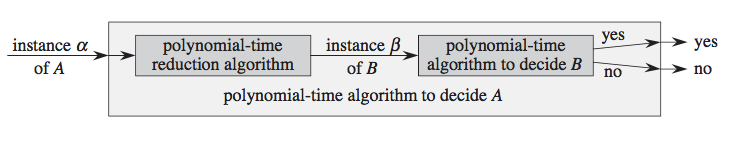
\includegraphics[width=\textwidth]{reduction.png}
            \item To solve $A$ in polynomial time, we reduce problem $A$ to $B$
            \begin{enumerate}
                \item Given an instance $\alpha$ of problem $A$, use reduction algorithm to transform it into an instance $\beta$ of $B$ 
                \item Run polynomial-time decision algorithm for $B$ on instance $\beta$
                \itme Use answer for $\beta$ as answer for $\alpha$
            \end{enumerate}
            \item \textbf{Usage} We can use polynomial time reduction in opposite way to \textbf{show that a problem is NPC}. Given a decision problem $A$ for which we know no polynomial-time algorithm can exist and a polynomial-time reduction algorithm that transforms instanaces of $A$ to instances of $B$. Then no polynomial-time algorithm exists for $B$
            \begin{proof}
                 Proof by contradiction. Suppose that otherwise $B$ has polynomial time algorithm, then along with the polynomial time reduction algorithm, we would have an algorithm (polynomial-time Algo for reducing $A$ to $B$ and deciding $B$) that solves $A$ in polynomial time, which contradicts assumption. 
            \end{proof}
            The catch is we cannot be sure there is no polynomial-time algorithm for $A$. So we prove $B$ is NPC on the assumption that problem $A$ is also NPC.
        \end{enumerate}
        \item \textbf{A first NP-complete problem}
        We need a first NPC problem to prove a different problem as NPC with reduction. The problem is the \textbf{circuit-satisfiability} problem, in which we are given a boolean combinational circuit composed of AND, OR, and NOT gates, and wich to know if there exists some set of boolean inputs to this circuit that causes its output to 1.
    \end{enumerate}
\end{defn*}


\subsection*{34.1 Polynomial time}


\begin{defn*}
    We consider polynomial time solvable problem tractible for philosophical reasons
    \begin{enumerate}
        \item Many problem has a small exponent $O(n^c)$ where $c$ is relatively small
        \item polynomial-time solvable problems usually remains solvable in polynomial time cross different models of computations (random-access machine, turing machine, parallel computer)
        \item polynomials are closed under addition, multiplication, and composition, i.e. composite polynomial-time algorithm remains to be polynomial
    \end{enumerate}
\end{defn*}

\begin{defn*}
    \textbf{Abstract Problems} 
    \begin{enumerate}
        \item \textbf{Abstract problem} $Q$ is a binary relation on a set $I$ of problem \textbf{instances} and a set $S$ of problem \textbf{solutions}. (i.e. an instance for \textsc{Shortest-Path} is a triple $(G, u, v)$, with solution as a sequence of vertices in graph. The problem itself is the relation that associates each instance to a shortest path in graph connecting the two vertices)
        \item \textbf{Decision problem} is a function that maps the instance set $I$ to the solution set $\{ 0, 1\}$ (i.e. for decision problem \textsc{Path}, if $i = \langle G, u, v, k \rangle$ is an instance, then $\textsc{Path}(i) = 1$ (yes) if a shortest path from $u$ to $v$ has at most $k$ edges, and $0$ (no) otherwise)
        \item \textbf{Optimization problem} in which require some value to be minimized or maximized. We can recast an optimization problem as a decision problem that is no harder.
    \end{enumerate}
\end{defn*}


\begin{defn*}
    \textbf{Encoding}
    \begin{enumerate}
        \item \textbf{Encoding} of a set $S$ of abstract objects is a mapping $e$ from $S$ to thet set of binary strings. 
        \begin{enumerate}
            \item Computer programs solves abstract decision problem by taking an encoding of a problem instance as input.
            \item We use encodings to map abstract problems to concrete problems. Given an abstract decision problem $Q: I \to \{0,1\}$, an encoding $e: I \to \{0, 1 \}^*$ can induce a related concrete decision problem, which we denote $e(Q)$. If solution to abstract instance $i\in I$ has solution $Q(i) \in \{0, 1\}$, then solution to the concrete problem instance $e(i)\in \{ 0, 1\}^*$ is also in $Q(i)$
            \item The concrete problem produces the same solutions as the abstract problem on binary-string instances that represent the encodings of abstract-problem instances.
        \end{enumerate}
        \item \textbf{Concrete Problem} A problem whose instance set $I$ is the set of binary strings. 
        \item An algorithm \textbf{solves} a concrete problem in $O(T(n))$ if when it is provided a problem instance $i$ of length $n = |i|$, the algorithm can produce the solution in $O(T(n))$ time. 
        \item \textbf{Polynomial-time solvable} A concrete problem for which there exists an algorithm to solve it in $O(n^k)$ for some constant $k\in \R$
        \item \textbf{Complexity class $P$} is a set of concrete decision problems that are polynomial-time solvable.
        \item \textbf{Polynomial-time computable} A function $f: \{0,1\}^* \to \{0,1\}^*$ is polynomial-time computable if there exists a polynomial-time algorithm $A$ that, given any input $x \in \{ 0, 1\}^*$, produces as output $f(x)$. 
        \item \textbf{Polynomially related} Two encoding $e_1$ and $e_2$ are polynomial related if there exists two polynomial-time computable function $f_{12}$ and $f_{21}$ such that for any $i\in I$ we have $f_{12}(e_1(i)) = e_2(i)$ and $f_{21}(e_2(i)) = e_1(i)$. That is a polynomial time algorithm can compute the encoding $e_2(i)$ from encoding $e_1(i)$ and vice versa 
    \end{enumerate}
\end{defn*}


\begin{lemma*}
    Let $Q$ be an abstract decision problem on instance set $I$, and let $e_1$ and $e_2$ be polynomially related encodings on $I$. Then $e_1(Q) \in P$ if and only if $e_2(Q) \in P$
\end{lemma*}


\begin{defn*}
    \textbf{A formal-language framework} 
    \begin{enumerate}
        \item \textbf{Alphabet} $\Sigma$ is a finite set of symbols 
        \item \textbf{Language} $L$ over $\Sigma$ is any set of strings made up of symbols from $\Sigma$ (i.e. if $\Sigma = \{0,1\}$, the set $L = \{ 10, 11, 101, 111\}$ is a language of binary representation of binary numbers) 
        \item \textbf{empty string} denoted by $\epsilon$. \textbf{empty language} denoted by $\emptyset$ and \textbf{language of all strings} over $\Sigma$ is denoted by $L = \Sigma^*$
        \item \textbf{Complement} $\overline{L} = \Sigma^* \setminus L$
        \item \textbf{Concatenation} $L_1 L_2 = \{ x_1 x_2 : x_1\in L_1 \land x_2\in L_2\}$
        \item \textbf{Closure (kleene star)} of a language $L$ is $L^* = \{ \epsilon\} \cup L \cup L^2 \cup \cdots$, where $L^k$ is concatenation of $L$ to itself $k$ times
        \item For any decision problem $Q$, we have the set of instances represented by $\Sigma^*$ where $\Sigma = \{0, 1\}$. Since $Q$ is entirely characterized by input instances that produce a 1 (yes) we have 
        \[
            L = \{ x \in \Sigma^* : Q(x) = 1 \}
        \]
        For example, \textsc{Path} has the corresponding language 
        \begin{align*}
             \textsc{Path} = \{ \langle G, u, v, k\rangle: 
                &G \text{ undirected graph}\\
                &u,v\in V\\
                &k \in \mathbb{Z}\\
                &\text{exists path from $u$ to $v$ in $G$} \\
                &\text{consisting of at most $k$ edges} \} \\ 
        \end{align*}
        \item An algorithm $A$ \textbf{accepts} a string $x\in \{0,1\}^*$ if given input $x$, the algorithm's output $A(x)$ is 1. The language accepted by algorithm $A$ is the set of strings $L = \{x\in\{0,1 \}^*: A(x)=1 \}$. An algorithm $A$ \textbf{rejects} a string $x$ if $A(x) = 0$
        \item A language $L$ is \textbf{decided} by an algorithm $A$ if \textbf{every binary string in} $L$ is accepted by $A$ and every binary string not in $L$ is rejected by $A$
        \item A language $L$ is \textbf{accepted in polynomial time} by algorithm $A$ if it is accepted by $A$ and if in addition there exists a constant $k$ such that for any length-n string $x\in L$, algorithm $A$ accepts $x$ in time $O(n^k)$
        \item A language $L$ is \textbf{decided in polynomial time} by an algorithm $A$ if there exsits a constant $k$ such that for any length-n string $x\in \{ 0,1\}^*$, the algorithm correctly decides if $x\in L$ in time $O(n^k)$ (so an algorithm accepting a language needs only produce answer when provided string in $L$, but must accept or reject every string in $\{0,1 \}^*$ if were to decide a language)
        \item \textbf{alternative definition for class $P$}
        \[
            P = \{L \subseteq \{0,1\}^*: \text{ exists algorithm $A$ that decides $L$ in polynomial time} \}
        \]
    \end{enumerate}
\end{defn*}


\subsection*{34.2 Polynomial-time verification} 


\begin{example}
    For \textsc{Path} problem, we can check if a certificate $p$ in $G$ has length of at most $k$. Verifying the certificate can be done in linear time, which takes as long as solving the problem from scratch (\textsc{Path}). Since $\texsc{Path} \in P$, so verifying a certificate doesnt buy much time. But there are problems with no polynomial time algorithm for which verifying a certificate is easy.
\end{example}

\begin{defn*}
    \textbf{Hamiltonian cycles} 
    \begin{enumerate}
        \item A \textbf{Hamiltonian cycle} of an undirected graph $G = (V,E)$ is a simple cycle that contains each vertex in $V$. \\
        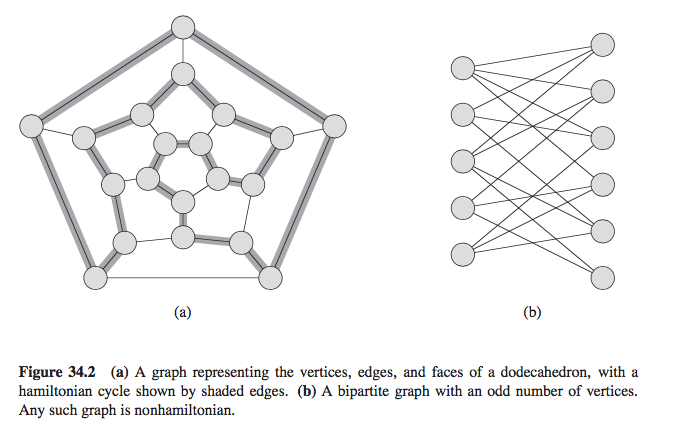
\includegraphics[width=\textwidth]{hamiltonian}
        \item A graph containing a hamiltonian cycle is \textbf{hamiltonian}(dodecahedron), otherwise it is \textbf{nonhamiltonian}. 
        \item \textbf{Hamiltonian cycle problem} asks if a graph $G$ have a hamiltonian cycle
        \[
            \textsc{HAM-CYCLE} = \{ \langle G \rangle: \text{ $G$ is a hamiltonian graph } \}
        \]
        \item \textbf{Permutation algorithm} list all permutation of vertices of $G$, check each permutation to see if its a hamiltonian path. Runs in exponential time $\Omega(2^{\sqrt{n}})$
    \end{enumerate}
\end{defn*}

\begin{defn*}
    \textbf{Verification algorithm} 
    \begin{enumerate}
        \item \textbf{Verification algorithm} is a two-argument algorithm $A$, where one argument is an ordinary input string $x$ and the other is a binary string $y$ called \textbf{certificate}
        \item $A$ \textbf{verifies} an input string $x$ if there exists a certificate $y$ such that $A(x,y) = 1$. 
        \item The \textbf{language verified} by a verification algorithm $A$ is 
        \[
            L = \{ x\in \{ 0,1\}^*: \text{ there exists } y\in \{0,1 \}^* \text{ such that } A(x,y) = 1 \}
        \]
        \item Given a sequence of vertiecs (path), its easy to verify if the cycle is hamiltonian by checking whether 
        \begin{enumerate}
            \item it is a permutation of the vertices of $V$
            \item consecutive edges along the cycle actually exists in graph $G$
        \end{enumerate}
        The algorithm can be impl in $O(n^2)$ time. The certificate to the problem is a list of vertices in some hamiltonian cycle. If a graph is hamiltonian, the cycle itself can be verified. 
    \end{enumerate}
   
\end{defn*}

\begin{defn*}
    \textbf{Complexity class NP}
    \begin{enumerate}
        \item \textbf{NP} is the class of languages that can be verified by a polynomial time algorithm. More preciesely, a language $L$ belongs to $NP$ if and only if there exists a two-input polynomial-time algorithm $A$ and a constant $c$ such that 
        \[
            L = \{x\in \{ 0,1\}^* : \text{ there exists a certificate $y$ with $|y| = O(|x|^c)$ such that $A(x,y) = 1$ } \}
        \]
        \item We say that algorithm $A$ \textbf{verifies} the language $L$ in polynomial time
        \item $\textsc{Ham-Cycle} \in NP$
        \item if $L\in P$ then $L\in NP$, i.e. $P\subseteq NP$ (decidability implies verifiability)
        \begin{proof}
            If there is a polynomial time algorithm to decide $L$, the algorithm can be converted to a two-argument verification algorithm that ignores any certificates and accepts exactly those input strings it determines to be in $L$ (i.e. just use the decision algorithm's output as verification)
        \end{proof}
        \item Unknown if $P = NP$, most believe they are not same class ($\exists L \in NP$ s.t. $L\not\in P$). Its intuitive to think that its more difficult to solve a problem from scratch than to verify a clearly presented solution.
        \item \textbf{co-NP} is a complexity class such that a problem $L \in \textsc{co-NP}$ if and only of $\overline{L} \in NP$. It is a class of problems for which there is a polynomial-time algorithm that can verify \textbf{no} instances 
        \item There is another open question as to if $NP$ is closed under complement, i.e. if $NP = \textsc{co-NP}$
        \item $P$ is closed under complement.
    \end{enumerate}
\end{defn*}


\begin{theorem*}
    $P\subseteq \textsc{co-NP}$
\end{theorem*}

\subsection*{NP-Completeness and Reducibility}



\begin{defn*}
    \textbf{Intuition}
    \begin{enumerate}
        \item belief in $P\neq NP$ comes from existence of NPC problems
        \item If \textbf{any} NPC problem can be solved in polynomial time, then \textbf{every} problem in NP can be solved in polynomial-time
        \item \textsc{Ham-Cycle} is a NPC problem. If we can decide \textsc{Ham-Cycle} in polynomial time, then we could solve every problem in NP in polynomial time. Moreover, if $NP-P\neq \emtpyset$, then \textsc{Ham-Cycle} $\in NP - P$
        \item NPC problems are the hardest language in $NP$. 
    \end{enumerate}
\end{defn*}



\begin{defn*}
    \textbf{Reducibility} 
    \begin{enumerate}
        \item a problem $Q$ can be reduced to another problem $Q'$ if any instance of $Q$ can be easily rephrased as an instance of $Q'$, the solution to which provides a solution to the instance of $Q$. $Q$ in a sense is \textbf{no harder to solve} than $Q'$
        \item \textbf{polynomial-time reducible} A langauge $L_1$ is polynomial-time reducible to a language $L_2$, written $L_1 \leq_p L_2$ if there exists a polynomial-time computable function $f: \{ 0,1\}^* \to \{ 0,1\}^*$ such that for all $x\in  \{ 0,1\}^*$, $x\in L_1$ if and only if $f(x)\in L_2$. 
        \begin{enumerate}
            \item The function $f$ is the \textbf{reduction function}. The reduction function provides a polynomial-time mapping such that if $x\in L_1$ then $f(x)\in L_2$ and if $x_2\not\in L_1$ then $f(x) \not\in L_2$ 
            \item The reduction function maps any instance $x$ of the decision problem represented by language $L_1$ to an instance $f(x)$ of the problem represented by $L_2$. Implying providing an answer to whether $f(x)\in L_2$ directly provides the answer to whether $x\in L_1$
            \item a polynoimal-time algorithm $F$ that computes $f$ is a \textbf{reduction algorithms}
        \end{enumerate}
        \item Polynomial-time reductions provide a formal means for showing that one problem is at least as hard as another, to within a polyonmial-time factor.
        \[
            \text{If $L_1 \leq_p L_2$,then $L_1$ is not more than a polynomial factor harder than $L_2$}
        \]
    \end{enumerate}
\end{defn*}

\begin{lemma*}
    If $L_1, L_2 \subseteq \{0,1\}^*$ are languages such that $L_1 \leq_p L_2$, then $L_2 \in P$ implies $L_1 \in P$
    \begin{proof}
        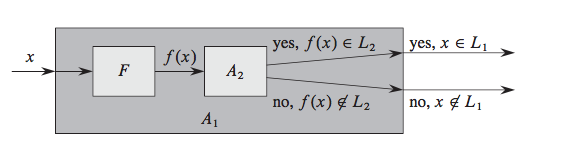
\includegraphics[width=\textwidth]{reducibility_lemma.png}
        Let $A_2$ be a polynomial-time algorithm that decides $L_2$, and let $F$ be a polynomial-time reduction algorithm that computes the reduction function $f$. Now we construct a polynomial-time algorithm $A_1$ that decides $L_1$. For any given input $x\in\{0,1\}^*$, algorithm $A_1$ uses $F$ to transform $x$ into $f(x)$ and then it uses $A_2$ to test whether $f(x)\in L_2$. The algorithm $A_1$ takes the output from algorithm $A_2$ and produces that answer as its own output. The correctness follows from the previous lemma. $x$ and $f(x)$ are two different encodings of problem $Q$ connected by a polynomial-time related encodings. Therefore, the solution set for $A_2$ is the solution set for $A_1$
    \end{proof}
\end{lemma*}

\begin{defn*}
    \textbf{NP-completeness}
    \begin{enumerate}
        \item \textbf{NP-completeness} A language $L\subseteq \{0,1\}^*$ is NPC if
        \begin{enumerate}
            \item $L\in NP$ 
            \item $L' \leq_p L$ for every $L' \in NP$ (NP-hard)
        \end{enumerate}
        \item \textbf{NP-hard} A language that satisfies second property but not necessarily first property, then $L$ is NP-hard.
        \item A proof that a problem is NPC provides that it is intractible
        \item We need to prove at least 1 problem as NPC, then we use polynomial-time reducibility as a tool to prove other problems to be NPC
    \end{enumerate}
\end{defn*}


\begin{theorem*}
    If any NP-complete problem ($NPC$) is polynomial-time solvable, then $P=NP$. Equivalently, if any problem in NP is not polynomial-time solvable, then no NP-complete problem is polynomial-time solvable.
    \begin{proof}
        Suppose $L\in P$, and also $L\in NPC$. For any $L' \in NP$, we have $L' \leq_p L$. By previous lemma, since $L\in P$ we have $L' \in P$. Therefore if any NPC $L$ is polynomial-time solvable, we can reduce every $NP$ problem to $L$ and solve them in polynomial-time. Hence $P\subseteq NP$ and $NP\subseteq P$ therefore $P=NP$. This prove the first statement. The second statement is contrapositive of the first.
    \end{proof}
\end{theorem*}

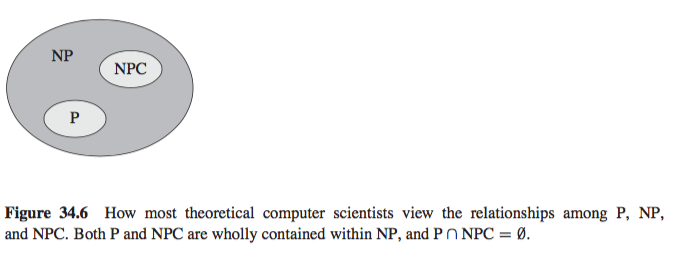
\includegraphics[width=\textwidth]{npc_venn.png}



\begin{defn*}
    \textbf{Circuit satisfiability} 
    \begin{enumerate}
        \item \textbf{the first proved NPC problem}
        \item \textbf{boolean combinational element} any circuit element that has a constant number of boolean inputs and outputs that performs a well-defined function
        \item \textbf{logic gates} are boolean combinational elements in circuit satisfiability problem (NOT, AND, OR gates). We can describe operation of each gates with a \textbf{truth table}
        \item \textbf{boolena combinational circuit} a circuit consisting of one or more boolean combinational elements interconnected by \textbf{wires}. A wire can connect the output of one element to input of another
        \begin{enumerate}
            \item contains no cycles 
            \item \textbf{Fan-out} is greatest number of inputs of gates of the same type to which the output can be safely connected.
            \item \textbf{circuit input} If no element output is connected to a wire, the wire is a circuit input
            \item \textbf{circuit output} If no element input is connected to a wire, the wire is a circuit output
        \end{enumerate}
        \item \textbf{truth assignment} A truth assignment for a boolean combinational circuit is a set of boolean input values 
        \item \textbf{satisfiable} A one-output boolean combinational circuit is satisfiable if it has a satisfying assignment: a truth assignment that causes the output of the circuit to be 1
        \item \textbf{circuit satisfiability problem} Given a boolean combinational circuit composed of AND, OR, NOT gate and ask if it is satisfiable. 
        \item \textbf{Naive solution} Check all possible assignments ($2^n$) to inputs ($n$) and see if at least one is a truth assignment that causes output to be 1.
        \item \textbf{Configuration} Computer's memory holds entire state of computation (program, program counter, storage, ...) Any particular state of an instruction is a configuration. Execution of an instruction is a mapping from one configuration to another 
    \end{enumerate}
\end{defn*}



\begin{lemma*}
    The circuit-satisfiability problem belongs to the class NP 
    \begin{proof}
        We shall provide a two-input, polynomial-time algorithm $A$ that can verify \textsc{Circuit-SAT}. 
        \begin{enumerate}
            \item One of the inputs to $A$ is an encoding of boolean combinational circuit $C$.
            \item The other being a \textbf{certificate} corresponding to an assignment of boolean values to wires in $C$.
        \end{enumerate}
        Construct algorithm $A$ as follows 
        \begin{enumerate}
            \item For each logic gates, checks value provided by certificate on each output wire provided by the certificate is computed correcty as a function of values on input wires
            \item If output of entire circuit is 1, then the algorithm outputs 1. Otherwise 0.
        \end{enumerate}
        For any satisfiable circuit $C$ as input to $A$ there exists a certificate whose length is polynomial in size of $C$ and that causes $A$ to output a 1. Whenever an unsatisfiable circuit is input, no certificate can fool $A$ into believing that the circuit is satisfiable. $A$ runs in polynomial time. Hence we can verify \textsc{Circuit-SAT} in polynomial-time, hence \textsc{Circuit-SAT} $\in NP$
    \end{proof}
\end{lemma*}



\begin{lemma*}
    The circuit-satisfiability problem is NP-hard 
    \begin{proof}
        Want to prove that $L \leq_p \textsc{Circuit-SAT}$ for every $L\in NP$. Let $L$ be any language in $NP$, we now describe a polynomial-time algorithm $F$ computing a reduction function $f$ that maps every binary string $x$ to a circuit $C = f(x)$ such that $x\in L$ if and only if $C \in \textsc{Circuit-SAT}$. Since $L\in NP$, then must exists algorithm $A$ that verifies $L$ in polynomial time. Let $T(n)$ be worst case running time of algorithm $A$ on length-$n$ input string and let $k\geq 1$ be a constant such that $T(n) = O(n^k)$ and length of the certificate is $O(n^k)$. The verification algorithm $A$ can be represented as a sequence of configurations. Each configuration can consists of 
        \begin{enumerate}
            \item program for $A$
            \item proram counter
            \item auxiliary machine 
            \item input $x$
            \item certificate $y$
            \item working storage 
        \end{enumerate}
        The boolean combinational circuit $M$ maps each configuration $c_i$ to the next $c_{i+1}$ starting at initial configuration $c_0$. $A$ writes the output (0 or 1) to a designated location and the value never changes afterwards. So if the algorithm runs for at most $T(n)$ steps, the output appears as one of the bits in $c_{T(n)}$. \\
        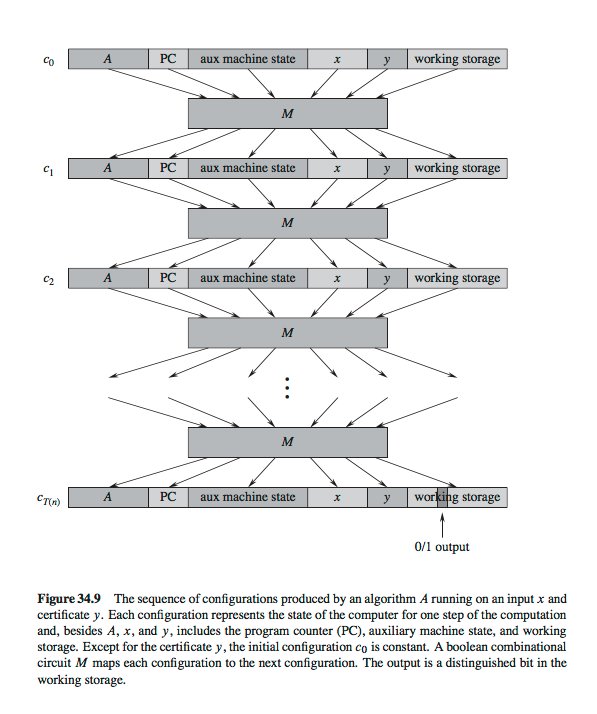
\includegraphics[width=\textwidth]{circuit_sat_nphard.png}
        The reduction algorithm $F$ works by constructing a single combinational circuit that computes all configurations by a given initial state. Idea is to paste together $T(n)$ copies of circuit $M$. The output of $i$-th circuit feeds to input of $(i+1)$-th circuit. So configurations, rather than being stored in memory, simply reside as values on wires connecting copies of $M$. Now we prove that the reduction algorithm $F$ computes a circuit $C = f(x)$ that is satisfiable if and only if there exists a certificate $y$ such that $A(x,y) = 1$. When $F$ obtains input $x$, it computes $n=|x|$ and constructs a combinational circuit $C'$ consisting of $T(n)$ copies of $M$. The input to $C'$ is an initial configuration corresponding to a computation on $A(x,y)$ and output is configuration $c_{T(n)}$. $F$ modifies upon $C'$ to construct $C = f(x)$ by 
        \begin{enumerate}
            \item wiring inputs to $C'$ corresponding to the program for $A$. the initial PC, input $x$, initial state of memory, and also a certificate $y$. 
            \item ignores all outputs from $C'$, except for the one bit of $c_{T(n)}$ corresponding to output of $A$. 
        \end{enumerate}
        The resulting circuit $C$ computes $C(y) = A(x,y)$ for any input $y$ of length $O(n^k)$. Now we need to prove that 
        \begin{enumerate}
            \item $F$ correctly computes a reduction function $f$, i.e. show $C$ is satisfiable if and only if there exists a certificate such that $A(x,y)=1$
            \begin{proof}
                Suppose there exists a certificate $y$ of length $O(n^k)$ such that $A(x,y)=1$. Then if apply the bits of $y$ to inputs of $C = f(x)$, the output of $C$ is $C(y) = A(x,y) = 1$. So if a certificate exists, then $C$ is satisfiable. For other direction, suppose $C$ is satisfiable. Then there exists an input $y$ to $C$ such that $C(y) = 1$, from which we conclude $A(x,y)=1$
            \end{proof}
            \item Show $F$ runs in polynomial time.
            \begin{proof}
                the number of bits required to represent a configuration is polynomial in $n$. 
                \begin{enumerate}
                    \item The program for $A$ itself has constant size, independent of length of its input $x$
                    \item length of input $x$ is $n$
                    \item length of certificate $y$ is $O(n^k)$
                    \item Since algorithm runs for at most $O(n^k)$ steps (verifier), the amount of work storage is polynomial in $n$ as well
                \end{enumerate}
                The combinational circuit $M$ implementing the hardware has size polynomial in length of a configuration, which is $O(n^k)$ hence size of $M$ is polynomial in $n$. Since $C$ consists of at most $t=O(n^k)$ copies of $M$, the reduction algorithm $F$ can construct $C$ from $x$ in polynomial time. 
            \end{proof}
        \end{enumerate}
        So language \textsc{Circuit-SAT} is at least as hard as any language in NP. This is because we have directly reduced any language $L\in NP$ to \textsc{Circuit-SAT} 
    \end{proof}
\end{lemma*}


\begin{theorem*}
    The circuit-satisfiability problem is NP-complete 
\end{theorem*}


\subsection*{34.4 NP-completeness proofs}

\begin{lemma*}
    If $L$ is a language such that $L' \leq_p L$ for some $L' \in NPC$, then $L$ is NP-hard. If, in adidtion, $L\in NP$, then $L\in NPC$
    \begin{proof}
        Since $L'$ is NPC, for all $L''\in NP$ we have $L'' \leq_p L'$. By transitivity, we have $L'' \leq_p L' \leq_p L$, so shown $L$ is NP-hard. If $L\in NP$, we also have $L\in NPC$ by definition of NP-completeness.
    \end{proof}
\end{lemma*}


\begin{defn*}
    \textbf{NPC proof techniques} By previous lemma, by reducing a known NPC language $L'$ to $L$, we implicitly reduce every language in $NP$ to $L$. 
    \begin{enumerate}
        \item Prove $L\in NP$
        \item Prove $L$ is NP-hard, i.e. $L' \leq_p L$ for some $L' \in NPC$
        \begin{enumerate}
            \item Select a known NP-complete problem $L'$
            \item Describe an algorithm that computes a function $f$ mapping every instance $x\in \{0,1\}^*$ of $L'$ to an instance $f(x)$ of $L$
            \item Prove that the function $f$ satisfies $x\in L'$ if and only if $f(x)\in L$ for all $x\in \{0,1\}^*$
            \item Prove the algorithm computing $f$ runs in polynomial time.
        \end{enumerate}
    \end{enumerate}
\end{defn*}

\begin{defn*}
    \textbf{Formula Satisfiability} 
    \begin{enumerate}
        \item \textbf{truth assignment} for a boolean formula $\phi$ is a set of values for the variables of $\phi$ 
        \item \textbf{satisfying assignment} is a truth assignment that causes it to evaluate to 1
        \item \textbf{Satisfiable formula} is a formula with a satisfying assignment. 
        \item \textbf{Formula satisfiability problem} in terms language \textsc{SAT} as follows 
        \begin{enumerate}
            \item $n$ boolean variables $x_1, \cdots, x_n$ 
            \item $m$ boolean connectives: any boolean function with one or two inputs and one outputs, such as $\land$ $\lor$ $\neg$ $\to$ $\iff$ 
            \item parentheses.
        \end{enumerate} 
        We can encode a boolean formula $\phi$ in a length that is polynomial in $n+m$. We ask if whether a given boolena formula is satisfiable. 
        \[
            \textsc{SAT} = \{\langle \phi \rangle : \phi \text{ is satisfiable boolean formula }  \}
        \]
        \item \textbf{A naive exponential time algoriothm} Check every single assignment ($2^n$) for a formula $\langle \phi \rangle$ of $n$ variables. If length of $\langle \phi \rangle$ is polynomial in $n$, then checking every assignment requires $\Omega(2^n)$ time
    \end{enumerate}
\end{defn*}

\begin{theorem*}
    Satisfiability of boolean formulas is NP-complete
    Two part proof 
    \begin{enumerate}
        \item Prove $\textsc{SAT}\in NP$
        \begin{proof}
            Need to show that a certificate consisting of a satisfying assignment from an input formula $\phi$ can be verified in polynomial time. The verifying algorithm simply replaces each variable in the formula with its corresponding value and then evaluates the expression. This can be done in polynomial time. If the expression evaluates to 1, then algorithm has verified that the formula is satisfiable. Hence $\textsc{SAT}\in NP$
        \end{proof}
        \item Prove $\textsc{SAT}$ is NP-hard
        \begin{proof}
            We can prove this by showing that $\textsc{Circuit-SAT} \leq_p \textsc{SAT}$. In other words, we need to show a reduction algorithm that reduce any instance of circuit satisfiability to an instance of formula satisfiability in polynomial time. The reduction algorithm which look at the gates that produces the circuit output and inductively express each of gates' inputs as formulas does not work. The problem arise from shared-subformula, in which gates whose output wires have fan-out of 2 or more can cause size of generated formula to grow exponentially. Have to find a smarter solution. Each wire $x_i$ in circuit $C$ has a variable $x_i$. We express how each gates operate as a small formula invovling varaibles of its incident wires. (i.e. AND gate $z \iff (x \land y)$) These small formulas are \textbf{clauses} The reduction algorihtm generates formula $\phi$ as the AND of
            \begin{enumerate}
                \item circuit-output variable (output -> 1), and 
                \item conjunction of clauses describing operation of each gates (so that gate logic is valid)
            \end{enumerate}
            Now we show that circuit $C$ is satisfiable if and only if $\phi$ is satisfiable. If $C$ has a satisfying assignment, then each wire of circuit has a well-defined value, and output of circuit is 1. Therefore, when we assign wire values to variables to $\phi$, each clause of $\phi$ evaluates to 1, and thus conjunction of all clauses (for each gate) along with the final output evaluates to 1. Conversely, if some assignment causes $\phi$ to evaluate to 1, then circuit $C$ is satisfiable by an analogous argument. Hence $\textsc{Circuit-SAT} \leq_p \textsc{SAT}$
        \end{proof}
    \end{enumerate}
\end{theorem*}


\begin{defn*}
    \textbf{3-CNF satisfiability} 
    \begin{enumerate}
        \item \textbf{motivation} formula satisfiability is very useful in proving many other NPC problems. But reduction algorithm must handle any input formula and this can lead to many number of cases, so might want a restrricted langauge of boolean formulas
        \item \textbf{Literal} in a boolean formula is an occurrence of a variable or its negation. 
        \item \textbf{Conjunctive normal form (CNF)} A boolean formula is in conjunctive normal form if it is expressed as an AND of clauses, each of which is the OR of one or more literals. 
        \item \textbf{3-CNF} A boolean formula is in 3-CNF if each clause has exactly three distinct literals. For example
        \[
            (x_1 \lor \neg x_1 \lor \neg x_2) \land (x_3 \lor x_2 \lor x_4)
        \]
        \item \textbf{3-CNF satisfiability problem} Ask if a given boolean formula $\phi$ in 3-CNF is satisfiable. 
    \end{enumerate}
\end{defn*}


\begin{theorem*}
    Satisfiability of boolean formulas in 3-CNF is NP-complete 
    \begin{enumerate}
        \item Prove $\textsc{3-CNF-SAT} \in NP$
        \begin{proof}
            The certificate of the problem is a truth assignment for the input formula $\phi$. We provide the verifying algorithm as simply replacing each variable in the formula with values of the variable and evaluates the expression. This can be done in polynomial time. If the expression evalutes to 1, the algorithm verifies that the formula is satisfiable. Here we have shown that such algorithm can verify \textsc{3-CNF-SAT} in polynomial time
        \end{proof}
        \item Prove $\textsc{SAT} \leq_p \textsc{3-CNF-SAT}$
        \begin{proof}
            The reduction algorithm is as follows. 
            \begin{enumerate}
                \item We construct a binary parse tree for the input formula $\phi$, with literals as leaves and connectives as internal nodes. For cluases with more than 2 OR of literals, we can use associativity to parenthesize the expression fully so that every internal node in resulting tree has 1 or 2 children. Now similar to how we proved \textsc{SAT}, we rewrite $\phi$ as AND of the root variable and a conjunction of clauses describing the operation of each node (we introduce a variable $y_i$ as output of each internal node, output of root as being $y_i$) Observe that $\phi'$ obtained is a conjunction of clauses $\phi_i'$, each of which has at most 3 literals (2 children and internal node output).
                \item  Now we convert each clause $\phi'$ by evaluating all possible assignment to its variables. Write up truth table for each clause, and use rows in which outputs 0, we can rewrite the original clause in \textbf{disjunctive normal form (DNF)} or OR (handle different rows) of ANDs (handles a single row) of literals (input variables that may be either 1 or 0), which is equivalent to $\neg \phi_i'$. We negate DNF clauses and convert it into a CNF formula $\phi_i''$ by using demorgan's law to complement all literals, change ORs to ANDs, and change ANDs to ORs. Now we have converted each clause $\phi_i'$ of formula $\phi'$ into a CNF formula $\phi_i''$ and so $\phi'$ is equivalent to the CNF formula $\phi''$ and moreover each has at most 3 literals 
                \item Now we transform the formula so that each clause has exactly 3 clauses. The formula $\phi'''$ has 2 auxiliary variables $p$ and $q$/ For each cluase $C_i$ of $\phi''$, we 
                \begin{enumerate}
                    \item if $C_i$ has 3 distinct literals then simply include $C_i$ as a clause of $\phi'''$
                    \item If $C_i$ has 2 distinct literals, i.e. $C_i = (x_1 \lor x_2)$ then include $(x_1 \lor x_2 \lor p) \land (x_1\lor x_2 \lor \neg p)$ as clauses of $\phi'''$. Now matter values of $p$, one clause is evaluted to 1 and the other evalutes to $(x_1 \lor x_2)$
                    \item If $C_i$ has 1 distinct literal $x$ then include $(x \lor p \lor q) \land (x \lor p \lor \neg q) \land (x \lor \neg p \lor q ) \land (x\lor \neg p \lor \neg q)$ as clauses of $\phi'''$. Regardless values of $p$ or $q$, one of four clauses is equivalent to $x$ and the other 3 evaluates to 1.
                \end{enumerate}
            \end{enumerate}
            Now note 3-CNF formula $\phi'''$ is satisfiable if and only if $\phi$ is satisfiable. Each step preserves satisfiability. first step preserves satisfiability by construction of $\phi'$. second step CNF formula $\phi''$ is algebraically equivalent to $\phi'$. The 3-CNF formula $\phi'''$ is effectively equivalent to $\phi''$ since any assignment to $p$ and $q$ produces a formula that is algebraically equivalent.\\
            Additionally, we have to show the reduction can be computed in polynomial time 
            \begin{enumerate}
                \item construction of $\phi'$ from $\phi$ introduce at most 1 variable and 1 clause per connective in $\phi$. 
                \item construction of $\phi''$ from $\phi'$ introduce at most 8 clauses (since at most $2^3$ rows in a truth table with 3 inputs, and at most 3 literals in a clause) into $\phi''$ from $\phi'$
                \item construction of $\phi'''$ from $\phi''$ introduce at most 4 clauses (assuming it happens that each clause has only one literal) 
            \end{enumerate}
            So size of the resulting formula $\phi'''$ is polynomial in length of the original formula $\phi$. So each of the constructions can easily be reduced in polynomial time
        \end{proof}
    \end{enumerate}
\end{theorem*}


\subsection*{34.5 NP-complete problems} 

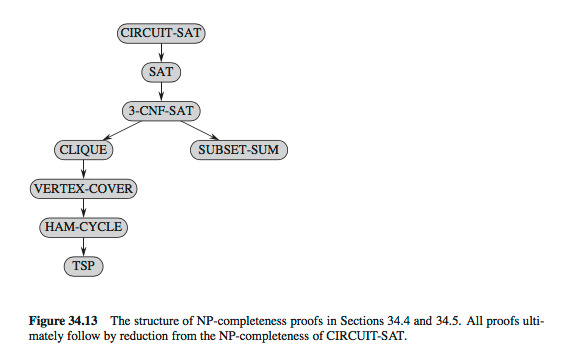
\includegraphics[width=\textwidth]{npc_proof_graph.png}


\begin{defn*}
    \textbf{The Clique problem}
    \begin{enumerate}
        \item \textbf{Clique} A clique in an undirected graph $G = (V,E)$ is a subset $V' \subseteq V$ of vertices, each pair of which is connected by an edge in $E$. In other words, a clique is a complete subgraph of $G$
        \item \textbf{Size of Clique} is the number of vertices it contains 
        \item \textbf{Clique problem} is an optimization problem of finding a clique of maximum size in a graph. As a decision problem. we ask whether a clique of a given size $k$ exsits in the graph
        \[
            \textsc{Clique} = \{\langle G, k \rangle: G \text{ is a grpah containing a clique of size } k \}
        \]
        \item \textbf{Naive super-polynomial algorithm} to the decision problem. List all $k$-subsets of $V$ and check each one to see whether if any one of them forms a clique. The running time is $\Omega (k^2 \binom{|V|}{k})$ ($k^2$ because need to check every edge in the subgraph induced by the $k$-subset) If $k$ is constant then runtime is polynomial. But in general, $k \sim \frac{|V|}{2}$, in which case the algorithm runs in superpolynomial time.
    \end{enumerate}
\end{defn*}

\begin{theorem*}
    \textbf{The clique problem is NP-complete}
    \begin{enumerate}
        \item Prove \textsc{Clique}$\in NP$ 
        \begin{proof}
            For a given graph $G = (V,E)$, use set $V'\subseteq V$ of vertices as a certificate for $G$. We can check whether $V'$ is a clique in polynomial time by checking whether, for each pair $u,v\in V'$, the edge $(u,v)$ belongs to $E$ 
        \end{proof}
        \item Prove $\textsc{3-CNF-SAT} \leq_p \textsc{Clique}$
        \begin{proof}
            The reduction algorithm begins with an instance of \textsc{3-CNF-SAT}. Let $\phi = C_1 \land C_2 \land \cdots \land C_k$ be boolean formula in 3-CNF with $k$ clauses. For $r = 1, 2, \cdots k$, each $C_r$ has exactly 3 distinct literals $l_1^r$, $l_2^r$, $l_3^r$. We now construct a graph $G$ such that $\phi$ is satisfiable if and only if $G$ has a clique of size $k$. The reduction algorithm works such that for each clause $C_r = (l_1^r, l_2^r, l_3^r)$ in $\phi$ place a triple of vertices $v_1^r$, $v_2^r$, $v_3^r$ into $V$, put an \textbf{edge between 2 vertices} $v_i^r$ and $v_j^s$ if both of following holds 
            \begin{enumerate}
                \item $v_i^r$ and $v_j^r$ are in different triples, i.e. $r\neq s$ and 
                \item their corresponding literals are consistent, i.e. $l_i^r$ is not he negation of $l_j^s$
            \end{enumerate}
            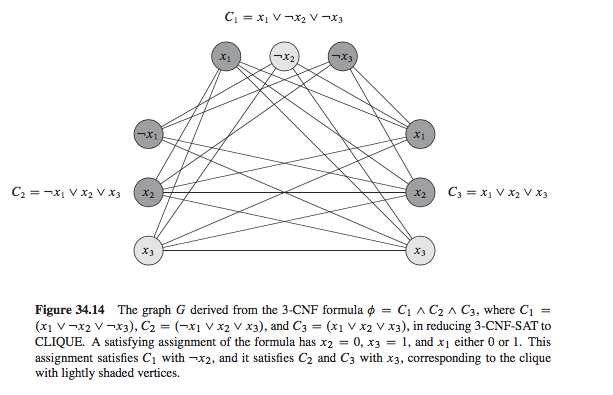
\includegraphics[width=\textwidth]{clique_proof.png}
            The reduction algorithm runs in polynomial time (easy to see). Now we have to show that the transformation from $\phi$ to $G$ is a reduction. Suppose $\phi$ has a satisfying assignment. Then each clause $C_r$ has at least one literal $l_i^r$ that is assigned 1, and each such literal corresponds to vertex $v_i^r$. Picking one such true literal from each clause yields a set $V'$ of $k$ vertices. Claim that $V'$ is a clique. For any two vertices $v_i^r, v_j^s\in V'$, where $r\neq s$, both corresponding literal $l_i^r$ and $l_j^s$ map to 1 by the given satisfying assignment, so the two literals cannot be complements. So by construction of $G$, edge $(v_i^r, v_j^s)$ belongs to $E$. Conversely, suppose $G$ has a clique $V'$ of size $k$. No edges in $G$ connect vertices in the same triple. So $V'$ contains exactly one vertex per triple. We can assign 1 to each literal $l_i^r$ such that $v_i^r \in V'$. Note this assignment cannot assign 1 to a literal and 0 to its complement, since $G$ contains no edges between inconsistent literals. Each clause is satisfied (by the fact that we have a $k$ clique) so $\phi$ is satisfied.\\
            Note the proof works on Clique of a particular structure, i.e. Clique is NP-hard only in graphs in which the vertices are restricted to occur in triples and that there are no edges between vertices in the same triple. But this is suffice to show that Clique is NP-hard in general graph as well. Since if we had a polynomial-time algorithm that sovles clique on the general graph, it would solve clique on restricted graph. \\
            Also reduction used the instance of \textsc{3-CNF-SAT} but not the solution. Since we cannot decide the solution to \textsc{3-CNF-SAT} in polynomial time, we cannot rely on knowing whether the formula $\phi$ is satisfiable.
        \end{proof}
    \end{enumerate}
\end{theorem*}



\subsection*{Vertex-Cover Problem}


\begin{defn*}
    \textbf{Vertex Cover Problem}
    \begin{enumerate}
        \item \textbf{Vertex Cover} of an undirected graph $G = (V,E)$ is a subset $V' \subseteq V$ such that if $(u,v)\in E$, then $u\in V'$ or $v\in V'$ or both. (every edge has at least 1 vertex in the cover) That is, each vertex covers its incident edges, and a vertex cover for $G$ is a set of vertices that covers all edges in $E$.
        \item \textbf{Size of vertex cover} is the number of vertices in it 
        \item \textbf{Vertex Cover problem} the optimization problem wants to find a vertex cover of minimum size in a given graph. The decision problem wants to determine if a graph has a vertex cover of a given size $k$. 
        \[
            \textsc{Vertex-Cover} = \{\langle G, k\rangle : \text{graph $G$ has a vertex cover of size $k$} \}
        \]
        \item \textbf{Complement of graph} The complement of $G$, $\overline{G} = (V,\overline{E})$ where 
        \[
            \overline{E} = \{ (u,v) : u,v\in V \quad \land \quad u\neq v \quad \land \quad (u,v)\not\in E \}
        \]
        In other words, the $\overline{G}$ contains exactly those edges that are not in $G$
    \end{enumerate}
\end{defn*}


\begin{theorem*}
    The vertex-cover problem is NP-complete
    \begin{enumerate}
        \item Prove $\textsc{Vertex-Cover}\in NP$ 
        \begin{proof}
            Given a graph $G = (V,E)$ and integer $k$, the certificate we choose is a vertex cover $V' \subseteq V$ itself. The verification algorithm checks 
            \begin{enumerate}
                \item $|V'| = k$ 
                \item for each edge $(u,v)\in E$, that $u\in V'$ or $v\in V'$ 
            \end{enumerate}
            This can be done in polynomial time easily.
        \end{proof}
        \item Prove \textsc{Vertex-cover} is NPC by showing $\textsc{Clique} \leq_p \textsc{Vertex-Cover}$
        \begin{proof}
            The reduction algorithm takes an input instance of \textsc{Clique} problem $\langle G, k\rangle$. The reduction computes the complement $\overline{G}$ and outputs an instance of $\langle \overline{G}, |V| - k\rangle$ of the \textsc{Vertex-Cover} problem. Now we prove that the transformation is a reduction: 
            \begin{center}
                the graph $G$ has a clique of size $k$ iff the graph $\overline{G}$ has a vertex cover of size $|V| - k$
            \end{center}
            \begin{enumerate}
                \item Suppose $G$ has a clique $V' \subseteq V$ with $|V'| = k$. We claim that $V - V'$ is a vertex cover in $\overline{G}$. Let $(u,v)\in \overline{E}$ be arbitrary. Then $(u,v) \not\in E$. This implies at least one of $u$ or $v$ does not belong to the clique subset $V'$, since every pair of vertices in $V'$ is connected by an edge of $E$. Equivalently, at least one of $u$ or $v$ is in $V - V'$ ($u,v\notin V' \to u,v\in V -V'$), this means that the edge $(u,v)$ is covered by $V-V'$. Since choice of $(u,v)$ is arbitrary, every edge of $\overline{E}$ is covered by a vertex in $V-V'$. set $V-V'$ has size $|V| - k$, which forms a vertex cover for $\overline{G}$
                \item Suppose $\overline{G}$ has a vertex cover $V'\subseteq V$, where $|V'| = |V| - k$. Then for all $u,v\in V$, if $(u,v) \in \overline{E}$ then $u\in V'$ or $v\in V'$ or both (by property of vertex cover). The contrapositive is that for all $u,v\in V$, if $u\not\in V'$ and $v\not\in V'$, the $(u,v)\in E$. In other words, $V-V'$ is a clique, with size $|V|- |V'| = k$
            \end{enumerate}
        \end{proof}
    \end{enumerate}
\end{theorem*}

\begin{defn*}
    \textbf{The hamiltonian-cycle problem}
    \begin{enumerate}
        \item A \textbf{Hamiltonian cycle} of an undirected graph $G = (V,E)$ is a simple cycle that contains each vertex in $V$. \\
        \item A graph containing a hamiltonian cycle is \textbf{hamiltonian}, otherwise it is \textbf{nonhamiltonian}. 
        \item \textbf{Hamiltonian cycle problem} asks if a graph $G$ have a hamiltonian cycle
        \[
            \textsc{HAM-CYCLE} = \{ \langle G \rangle: \text{ $G$ is a hamiltonian graph } \}
        \]
        \item \textbf{Permutation algorithm} list all permutation of vertices of $G$, check each permutation to see if its a hamiltonian path. Runs in exponential time $\Omega(2^{\sqrt{n}})$
    \end{enumerate}
\end{defn*}


\begin{theorem*}
    The hamiltonian cycle problem is NP-complete
    \begin{enumerate}
        \item Prove that $\textsc{Ham-Cycle}\in NP$
        \begin{proof}
            Given a graph $G = (V,E)$, a certificate is a sequence of $|V|$ vertices that make up the hamiltonian cycle. The verification algorithm checks 
            \begin{enumerate}
                \item the sequence contains each vertex $V$ eactly once 
                \item there is an edge between each pair of consecutive vertices and between the first and last vertex 
            \end{enumerate}
            The certificate can be verified in polynomial time
        \end{proof}
        \item Prove $\textsc{Vertex-Cover}\leq_p \textsc{Ham-Cycle}$
        \begin{proof}
            Given $\langle G, k \rangle$, we construt an undirected graph $G' = (V', E')$ that has a hamiltonian cycle if and only if $G$ has a vertex cover of size $k$. For each edge $(u,v)\in E$ the graph $G'$ will contain one copy of a \textbf{widget} (which enforces certain properties).  Denote each vertex in $W_{uv}$ by $[u,v,i]$ or $[v,u,i]$ where $1\leq i\leq 6$ (totals to 12 vertices)\\
            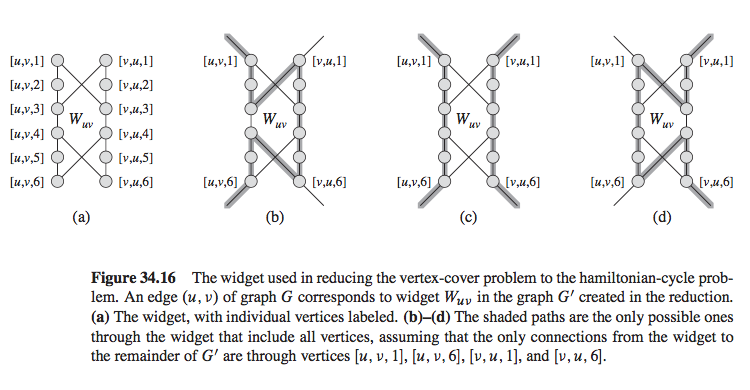
\includegraphics[width=\textwidth]{hamcycle_npc.png}
            \begin{enumerate}
                \item limit connection bewteen widget and remainder of graph $G'$, i.e. only $[u,v,1]$, $[u,v,6]$, $[v,u,1]$, $[v,u,6]$ will have edges incident from outside $W_{uv}$
                \item Every hamiltonian cycle must traverse edges of $W_{uv}$ in 3 possible ways
            \end{enumerate}
            We also include \textbf{selector vertices} $s_1,\cdots, s_k$. Use edges incident on selector vertices in $G'$ to select the $k$ vertices of the cover in $G$. \\ 
            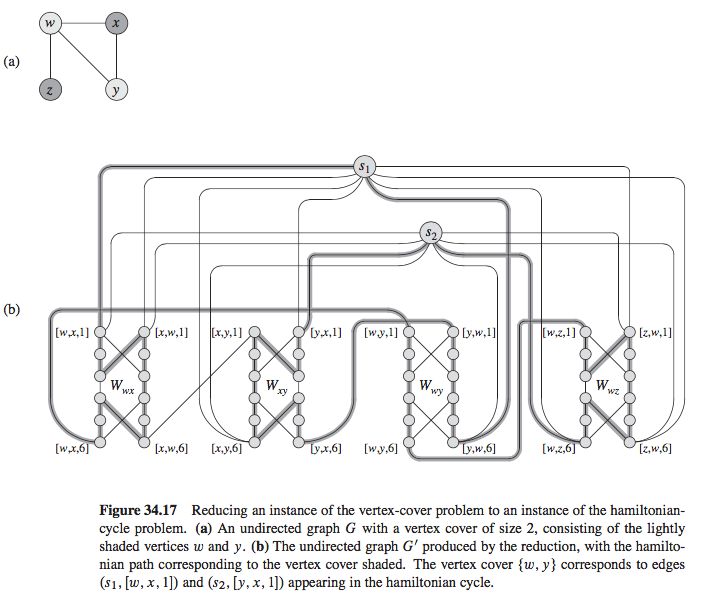
\includegraphics[width=\textwidth]{hamcycle_npc2.png}
            ...
        \end{proof}
    \end{enumerate}
\end{theorem*}


\begin{defn*}
    \textbf{Traveling salesman problem} Given a complete graph $G$ with $n$ vertices, a salesman wish to make a \textbf{tour} (hamiltonian cycle) visiting each vertex exactly once and finish at the starting vertex. For each $(i,j)\in E$, there is a nonnegative integer cost $c(i,j)$. The salesman wishs to make the tour whose total cost is minimum, where total cost is sum of individual costs along the edges of the tour 
    \begin{align*}
        TSP = \{\langle G, c, k \rangle : &G = (V,E) \text{ is a complete graph } \\
                    & \text{$c$ is a function from } V \times V \to \mathbb{Z}\\ 
                    & k\in \mathbb{Z} \\
                    & \text{$G$ has a traveling-salesman tour with cost at most } k \}\\
    \end{align*}
\end{defn*}


\begin{theorem*}
    \textbf{The traveling-salesman problem is NP-complete}
    \begin{enumerate}
        \item Prove $\textsc{TSP} \in NP$ 
        \begin{proof}
            Given an instance $\langle G, c, k \rangle$ or problem. The certificate is the sequence of $n$ vertices in the tour. The verification algorithm checks 
            \begin{enumerate}
                \item the sequence contains each vertex exactly once 
                \item sums summation of edge costs is at most $k$ 
            \end{enumerate}
            This can be done in polynomial time 
        \end{proof}
        \item Prove $\textsc{Ham-Cycle} \leq_p \textsc{TSP}$ 
        \begin{proof}
            Let $G = (V,E)$ be an instance of \textsc{Ham-Cycle}. Now we construct an instance of \textsc{TSP} as follows. We form the complete graph $G' = (V,E')$, where 
            \[
                E' = \{(i,j): i,j \in V \quad \text{and} \quad i\neq j \}
            \]
            with cost function function 
            \[
                c(i,j) = 
                \begin{cases}
                    0 & \text{if } (i,j)\in E\\
                    1 & \text{if } (i,j)\not\in E\\
                \end{cases}
            \]
            The instance of TSP is then $\langle G', c, 0 \rangle$. Note the transformation can be achieved in polynomial time. Now have to show that $G$ has a hamiltonian cycle if and only if $G'$ has a tour of cost at most 0. 
            \begin{enumerate}
                \item Suppose $G$ has a hamiltonian cycle $h$. Each edge in $h$ belongs to $E$ so has cost 0 in $G'$. Thus $h$ is a tour in $G'$ with cost 0. 
                \item Suppose $G'$ has a tour $h'$ of cost at most 0. Since the costs of edges in $E'$ are 0 or 1, the cost of tour $h'$ is exactly 0 implies each edge on the tour must have cost 0. Therefore $h'$ contains only edges in $E$, so $h'$ is a hamiltonian cycle in graph $G$
            \end{enumerate}
        \end{proof}
        \item Together TSP is NPC. Note that the instance of NPC is in a restricted form, in that $k$ is restricted to 0 and cost function $c$ takes value of 0 or 1 only. This is fine since if we know how to solve the generalized TSP problem, we can solve the restrited TSP problem. By contraposition, if we cant solve the restricted TSP problem, we cannot solve generalized TSP
    \end{enumerate}
\end{theorem*}

\begin{defn*}
    \textbf{Subset-sum problem} Given a finite set $S$ of positive integers and an integer \textbf{target} $t>0$. Ask whether there exists a subset $S' \subseteq S$ whose elements sum to $t$. 
    \[
        \textsc{Subset-Sum} = \{\langle S, t \rangle: \text{ there exists a subset $S' \subseteq S$ such that } t = \sum_{s\in S'} s \}
    \]
\end{defn*}




\begin{theorem*}
    The subset-sum problem is NP-complete
    \begin{enumerate}
        \item Prove $\textsc{Subset-Sum}\in NP$
        \begin{proof}
            Given an instance $\langle S, t\rangle$. Let $S'$ be the certificate. A verification algorithm simply sums up elements in $S'$ and check if it equates to $t$, which can be done in polynomial-time
        \end{proof}
        \item Prove $\textsc{3-CNF-SAT}\leq_p \textsc{Subset-Sum}$
        \begin{proof}
            Given a 3-CNF formula $\phi$ over $x_1, x_2, \cdots, x_n$ with clauses $C_1, \cdots, C_k$, each containing exactly 3 distinct literals. The reduction algorithm constructs an instance $\lange S, t \rangle$ such that $\phi$ is satisfiable if and only if there exists a subset of $S$ whose sum is $t$. The reduction construct $2n + 2k$ base 10 digits, each $n+k$ digits long, least significante $k$ digits are labelled by clauses and most significant $n$ digits are labled by variables 
            \begin{enumerate}
                \item target $t$ has 1 in each digit labeled by a variable and a 4 in each digit labled by a clause 
                \item For each $x_i$, set $S$ contains two integers $v_i$ and $v_i'$, with a 1 in the digit labeled by $x_i$ and 0s in other variable digits. If $x_i\in C_j$, then digit labeled by $C_j$ contains a 1. otherwise 0
                \item For each $C_j$, set $S$ contains 2 integers $s_j$ and $s_j'$ Each has 0 in all other digits other than the one labeled by $C_j$. For $s_j$ there is a 1 in $C_j$ digit, and for $s_j'$, there is a 2 in this digit. (slack variables)
            \end{enumerate}
            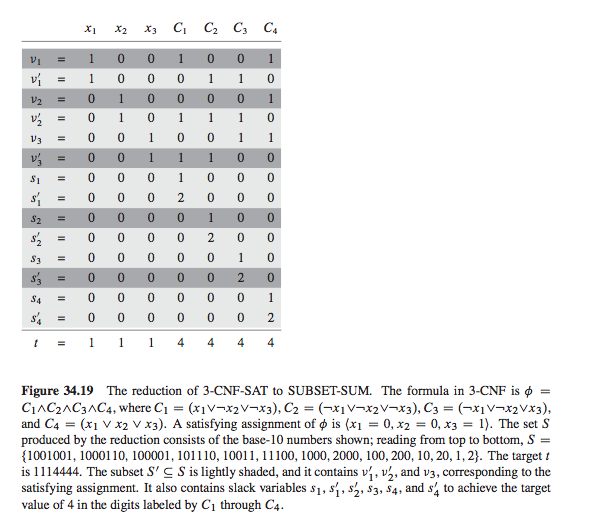
\includegraphics[width=\textwidth]{ss_npc.png} 
            The reduction can be done in polynomial time 
            \begin{enumerate}
                \item Suppose $\phi$ has a satisfying assignmen, For each $i$, if $x_i = 1$, then include $v_i$ in $S'$. Otherwise, include $v_i'$. So we include either $v_i$ or $v_i'$ for each $i$ but not both. We see that the variable digits sum up to 1s, which match $n$ most significant digits of $t$. Note since all cluase is satisfied, there must be a literal in each clause with value 1. Therefore, each digit labeled by a clause (least significant bits) has at least one 1 contributing to its sum by a $v_i$ or $v_i'$ value in $S'$. Since there can be 1,2,3 literals that are 1s, each clause digit has a sum of 1,2,or 3. We can chieve the target of 4 in each digit labeled by clause $C_j$ by including the appropriate nonempty subset of slack variables $\{s_j, s_j'\}$ in $S'$. So we have matched the target in all digits of the sum, the values of $S'$ sum to $t$. So $S'$ is a subset sum of $S$ given target $t$
                \item Suppose there is a subset $S' \subseteq S$ that sums to $t$. $S'$ must contain exactly one of $v_i$ and $v_i'$ for each $i = 1,\cdots, n$ for otherwise the sum would not be 1. If $v_i \in S'$, set $x_i$ to 1, otherwise $v_i' \in S'$, set $x_i$ to 0. Claim that every clause $C_j$ is satisfied by this assignment. Note to achieve a sum of 4 in digits labeled by $C_j$, there must be at least one of $v_i$ or $v_i'$ that has a 1 in the digit labeled by $C_j$, since inclusion of all slack $s_j$ and $s_j'$ sum to to 3 at most. If $v_i$ has a 1 in $C_j$'s position, then $x_i$ appear in clause $C_j$, clause $C_j$ is satisfied. Otherwise $S'$ includes a $v_i'$ that has a 1 in that position, then literal $\neg x_i$ appears in $C_j$. Since we set $x_i$ to 0 by the assignment scheme described earlier, clause $C_j$ is also satisfied. Thus all clauses $C_j$ is satisifed, this completes the proof
            \end{enumerate}
        \end{proof}
    \end{enumerate}
\end{theorem*}





\end{document}
